\documentclass[11pt,english,a4paper]{memoir}
\usepackage[T1]{fontenc}
\usepackage[utf8]{inputenc}

\usepackage{textcomp}

\usepackage[opticals,textosf,mathlf,swash,minionint,amsbb]{MinionPro}
\usepackage[final]{microtype}
\usepackage{pifont}

\usepackage{babel}
\usepackage{color}

\usepackage[hidelinks,final,bookmarksopen=true]{hyperref}

\hypersetup {
  pdftitle = {CV of Dr Heinrich Kuttler},
  pdfauthor = {Heinrich Kuttler}
}

\usepackage[absolute]{textpos}
\usepackage{graphicx}

\makeatletter

\settrimmedsize{297mm}{210mm}{*}
\setlength{\trimtop}{0pt}
\setlength{\trimedge}{\stockwidth}
\addtolength{\trimedge}{-\paperwidth}
\settypeblocksize{265mm}{157mm}{*}
\setulmargins{*}{*}{1}
\setlrmargins{*}{*}{1}
\setheadfoot{\onelineskip}{1.5\onelineskip}
\setheaderspaces{*}{\onelineskip}{*}
\checkandfixthelayout

\renewcommand{\footnoterule}{}
\setlength{\footmarkwidth}{-1.0em}
\setlength{\footmarksep}{-\footmarkwidth}
\footmarkstyle{#1~}
\renewcommand*{\@makefnmark}{\hbox{\textsuperscript{\@thefnmark}}}

\newcommand{\hairspace}{\kern .04167em}
\definecolor{Maroon}{cmyk}{0, 0.87, 0.68, 0.32}
\definecolor{halfgray}{gray}{0.55}
\definecolor{RoyalBlue}{cmyk}{1, 0.50, 0, 0}

\newcommand{\smallcaps}[1]{\textsc{\MakeLowercase{#1}}}

\copypagestyle{heinercv}{empty}
\makeoddfoot{heinercv}%
            {\color{halfgray}\footnotesize\smallcaps{CV of Heinrich
            Küttler, page \thepage\ of \thelastpage}}{}{}
\makeevenfoot{heinercv}%
             {\color{halfgray}\footnotesize\smallcaps{CV of Heinrich
             Küttler, page \thepage\ of \thelastpage}}{}{}
\pagestyle{heinercv}

\newcommand{\heinrichkuettleratgmaildotcom}{hein\rlap{\textcolor{white}{hugo@egon}}rich.kue\rlap{\textcolor{white}{@symmetry is overrated}}ttler@\rlap{\textcolor{white}{yesihatespamspamspam}}g\rlap{\textcolor{white}{spam@spam@spam!}}ma\rlap{\textcolor{white}{.de}}il.com}
\renewcommand{\heinrichkuettleratgmaildotcom}{hein\rlap{\textcolor{white}{ - }}rich.kue\rlap{\textcolor{white}{ }}ttler@\rlap{\textcolor{white}{}}g\rlap{\textcolor{white}{}}ma\rlap{\textcolor{white}{}}il.com}
\newcommand{\muelleratlmudotde}{mue\rlap{\textcolor{white}{hugo@egon}}ll\rlap{\textcolor{white}{@symmetry is overrated}}er@\rlap{\textcolor{white}{yesihatespamspamspam}}l\rlap{\textcolor{white}{spam@spam@spam!}}mu\rlap{\textcolor{white}{.com}}.de}
\newcommand{\heineratgoogledotcom}{hein\rlap{\textcolor{white}{hugo@egon}}e\rlap{\textcolor{white}{@symmetry is overrated}}r@\rlap{\textcolor{white}{yesihatespamspamspam}}g\rlap{\textcolor{white}{spam@spam@spam!}}oo\rlap{\textcolor{white}{.de}}gle.com}
\newcommand{\juergenvoigtattudresdende}{juer\rlap{\textcolor{white}{hugo@egon}}gen.voi\rlap{\textcolor{white}{@symmetry is overrated}}gt@\rlap{\textcolor{white}{yesihatespamspamspam}}tu-\rlap{\textcolor{white}{spam@spam@spam!}}dres\rlap{\textcolor{white}{.com}}den.de}

\newcommand{\uknumber}{+44~77\rlap{\textcolor{white}{666}}60~998\rlap{\textcolor{white}{456}}789}

\newcommand{\red}{\color{Maroon}}

\newcommand{\header}[1]{%
  \addlinespace[2ex]
  & \large{\red\textsc{\MakeLowercase{#1}}} \tabularnewline
  \midrule}

\newcommand{\n}{\tabularnewline}
\newcommand{\bull}{\Pisymbol{MinionPro-Extra}{146}~~}
\newcommand{\nobull}{\phantom{\bull}}

\newcommand{\Cpp}{C\kern-.03em\raise.16ex\hbox{\small{+\kern-.03em+}}}

\makeatother

\begin{document}

%% \begin{textblock*}{3.7cm}(135mm,17mm)
%%   %  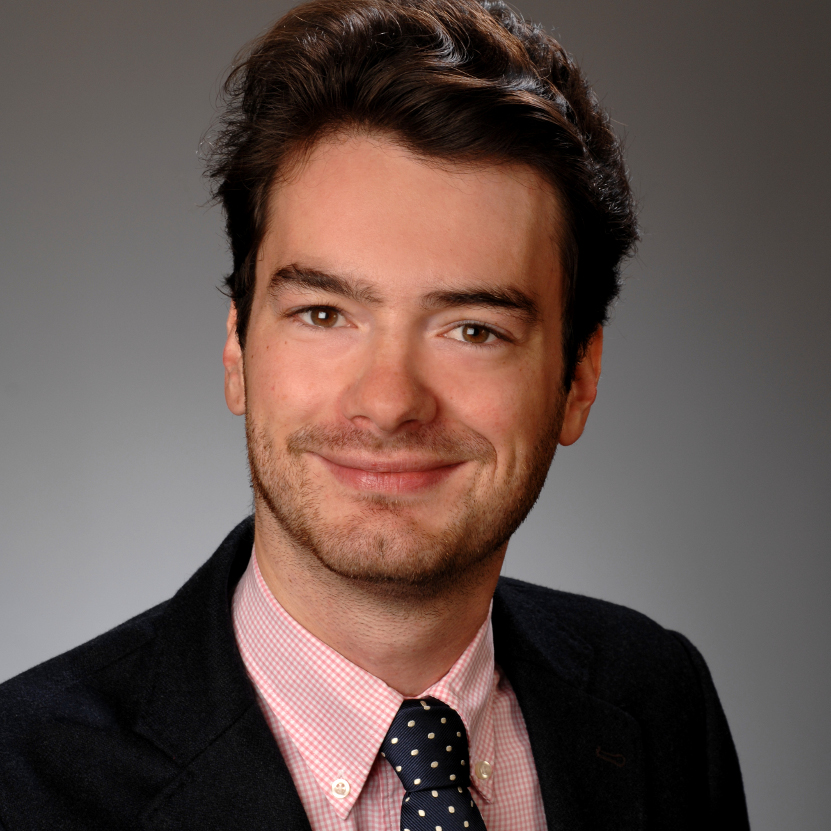
\includegraphics[width=3.7cm]{Foto_Heinrich_Kuettler_web.jpg}%
%% \begin{tabular}{rl}
%%   & \heinrichkuettleratgmaildotcom \n
%%   & +44 7760 998789 \n
%% \end{tabular}
%% \end{textblock*}

\begin{center}

\begin{tabular}{rl}
  & {\Large Dr Heinrich Küttler} \hspace\fill \heinrichkuettleratgmaildotcom
  \n & \hspace\fill \uknumber \n \addlinespace[0.5ex]

  \header{Experience}
  January 2019 & \textbf{Facebook AI Research, London} \n
  -- present & Research Engineer \n
  & \bull Lead researcher for large-scale RL research.

  \n \addlinespace
  July 2016 & \textbf{DeepMind, London} \n
  -- October 2018 & Senior Research Engineer, \ Team Lead \n
  & \bull Head of the DeepMind's \emph{Agents Team} and owner of the Reinforcement \\
  & \nobull Learning (RL) codebase for AI agents \\
  & \bull Winning DeepMind's internal \textit{AGI award} for
  large-scale multi-task \\
  & \nobull RL two cycles in a row (handed out by Shane Legg, founder, and Koray \\
  & \nobull Kavukcuoglu, Director of Research)

  \n \addlinespace
  July 2015 & \textbf{Google, London} \n
  -- July 2016 & Technical Solutions Consultant \n
  & \bull Built award-winning tool to analyse large amounts of advertising data, \\
  & \nobull used by 1000+ people within Google % \\
  % & \bull Responsibilities included identifying trends, providing strategic insights, \\
  % & \nobull and communicating growth directions to clients

  \n \addlinespace
  March 2010 & \textbf{LMU Munich, Germany} \n
  -- January 2015 & Research Assistant at the \href{http://www.mathematik.uni-muenchen.de/forschung/arbeitsgruppen/analysis/index.html}{Mathematics Institute} \n
  & \bull Teaching in several subjects,
  %(among them classical calculus, functional \\
  %& \nobull analysis, and complex analysis)
  %\\
  various talks and presentations in seminars \\ & \nobull and
  conferences

  %% \n \addlinespace
  %% August 2009      & \textbf{TU Munich, Germany} \n
  %% -- February 2010 & Research Assistant at the \href{http://www.lnm.mw.tum.de/}{Institute for Computational Mechanics} \n
  %% & \bull Development of finite element code in \Cpp\ for biofluid \\
  %% & \nobull mechanics applications, e.g., airflow in lung respiration

  \n
  \header{Education}
  March 2010        & \textbf{LMU Munich, Germany} \n
  -- September 2014 & PhD in Mathematical Physics \n
  & \bull Cumulative grade 0.9, \textit{magna cum laude} \n
  % & \nobull (Dissertation: 1.0, \textit{magna cum laude}, Disputation:
  % 0.7, \textit{summa cum laude}) \n
  & \bull Publications in highly-respected journals, including \textit{Comm. Math. Phys.}

  \n \addlinespace
  October 2004  & \textbf{TU Dresden, Germany} \n
  -- July 2009  & Major: Mathematics, \ Minor: Physics and Computer Science \n
  & \bull Diploma grade 1.0, with distinction \n
  & \bull Diploma exam included Functional Analysis, PDEs, Variational Calculus, \\
  & \nobull Probability Theory, OO programming, Computer Security and Cryptography

  %\n \addlinespace
  %July 2004 & \textbf{Peter-Breuer-Gymnasium, Zwickau, Germany} \n
  %& \bull German Abitur, cumulative grade 1.4

  \n
  \header{Internship}
  July 2008       & \textbf{University of Leicester, UK} \n
  -- August 2008  & Intern at the \href{http://www.le.ac.uk/biology/phh4/}{Department of Biology} \n
  & \bull Created software to analyse repetitive motifs in
  \textit{Drosophila} DNA, \\
  & \nobull leading to a publication in \textit{Mol. Biol. Evol.} (Oxford University Press)
  \n
  \header{Scholarships}
  Awarded & \textbf{German Academic Scholarship Foundation (Studienstiftung)} \n
  February 2007 & Grant awarded by Germany's most prestigious scholarship foundation
  \n
  & \bull Nomination based on undergraduate results (top 2\% of class
  eligible for \\
  & \nobull three-day selection seminar; \ $< 0.5\%$ of German students admitted)
\end{tabular}

\begin{tabular}{rl}
  \header{Skills}
  Languages & \bull German: native, \ English: fluent \n \addlinespace

  Coding
  & \bull Developed large-scale distributed machine learning frameworks in \n
  & \nobull PyTorch and TensorFlow (Python and \Cpp) \n
  & \bull Additional experience in TypeScript/JavaScript, Go, Java, Swift \\
  & \bull Released on Google Play App Store and other platforms

  \n
  \header{Other interests}

  & \bull Various Open Source projects
  (see \href{https://github.com/heiner}{github.com/heiner}) \n
  & \bull Amateur guitarist, typography enthusiast,
  hobby economist,  \\
  & \nobull and Bob Dylan aficionado

  \n
  \header{Publications}
  Machine Learning

  & \textit{TorchBeast: A PyTorch platform for distributed RL} \\
  and AI
  & Heinrich K{\"u}ttler, Nantas Nardelli, Thibaut Lavril, Marco
  Selvatici, \\
  & Viswanath Sivakumar Tim Rockt{\"a}schel, Edward Grefenstette \\
  & \href{https://arxiv.org/abs/1910.03552}{arXiv:1910.03552} \n \addlinespace

  & \textit{MVFST-RL: An Asynchronous RL Framework for Congestion
    Control} \\
  & \textit{with Delayed Actions} \\
  & Viswanath Sivakumar, Tim Rocktäschel, Alexander H. Miller, \\
  & Heinrich Küttler, Nantas Nardelli, Mike Rabbat, Joelle Pineau, \\
  & Sebastian Riedel \\
  & Workshop on ML for Systems at NeurIPS 2019; \ \href{https://arxiv.org/abs/1910.04054}{arXiv:1910.04054}
  \n \addlinespace

  & \textit{Kickstarting Deep Reinforcement Learning} \\
  & Simon Schmitt, Jonathan J. Hudson, Augustin Zidek, Simon Osindero, \\
  & Carl Doersch, Wojciech M. Czarnecki, Joel Z. Leibo, Heinrich Küttler, \\
  & Andrew Zisserman, Karen Simonyan, S. M. Ali Eslami \\
  & \href{https://arxiv.org/abs/1803.03835}{arXiv:1803.03835}
  \n \addlinespace

  & \textit{StarCraft II: A New Challenge for Reinforcement Learning} \\
  & Oriol Vinyals, et al (see \href{https://arxiv.org/abs/1708.04782}{arXiv:1708.04782}) \n \addlinespace

  & \textit{DeepMind Lab} \\
  & Charles Beattie, et al (see \href{https://arxiv.org/abs/1612.03801}{arXiv:1612.03801}) \n \addlinespace

  Mathematical Articles
  & \textit{The Exponent in the Orthogonality Catastrophe for Fermi Gases} \\
  & Martin Gebert, Heinrich Küttler, Peter Müller, Peter Otte \\
  & \href{http://dx.doi.org/10.4171/JST/135}{J. Spectr. Theory 6 (3), pages 643--683, European Math. Society, 2016} \n \addlinespace

  & \textit{Anderson's Orthogonality Catastrophe} \\
  & Martin Gebert, Heinrich Küttler, Peter Müller \\
  & \href{http://dx.doi.org/10.1007/s00220-014-1914-3}{Comm. Math. Phys. 329 (3), pages 979--998,
  Springer, 2014} \n \addlinespace

  & \textit{Anderson's Orthogonality Catastrophe for One-Dimensional Systems}
  \\
  & Heinrich Küttler, Peter Otte, Wolfgang Spitzer \\
  & \href{http://dx.doi.org/10.1007/s00023-013-0287-z}{Ann. Henri Poincaré \,15 (9), pages 1655--1696, Springer, 2014}

  \n \addlinespace
  Other peer-reviewed & \textit{The Repetitive DNA of Drosophila:
  Concerted Evolution at Different}
  \\
  articles & \textit{Genomic Scales and Association with Genes} \\
  & Gustavo C. S. Kuhn, Heinrich Küttler, Orlando Moreira-Filho, \\
  & John S. Heslop-Harrison \\
  & \href{http://dx.doi.org/10.1093/molbev/msr173}{Mol. Biol. Evol. 29 (1), pages 7--11, Oxford University Press, 2012}
  \n \addlinespace

  PhD thesis & \textit{Anderson's Orthogonality Catastrophe} \\
  & \href{http://edoc.ub.uni-muenchen.de/17442/}{LMU Munich, 2014} \n \addlinespace

  %% \n
  %% \header{Reference}
  %% PhD advisor & \textbf{Dr. Peter Müller}, Professor at Mathematics Institute, LMU München
  %% \\
  %% & Tel: +49 (0)89 2180\,4434, \ Email: \muelleratlmudotde

  %% \n \addlinespace

  %% Supervisor         & \textbf{Dr. Jürgen Voigt}, Professor at Department of
  %% Mathematics, TU Dresden \\
  %% for diploma thesis &
  %% Tel: +49 (0)351 463\,33790, \ Email: \juergenvoigtattudresdende
\end{tabular}

\end{center}

%%   \bigskip

%%   \hfill
%%   \includegraphics{signature}  \hspace*{-3.0em} \\
%%   \hspace*{\fill} Dr. Heinrich Küttler

\end{document}
